% M12 connector pin-out - Front view of computer-side connector
% Mirrored image of lidar-side: https://pdf.directindustry.com/pdf/velodynelidar/vlp-16-datasheets/182407-676097.html
% Author: Tobit Flatscher (https://github.com/2b-t)

\documentclass[border=10pt]{standalone}
\usepackage{tikz}
\usepackage{xintexpr}

\begin{document}
	
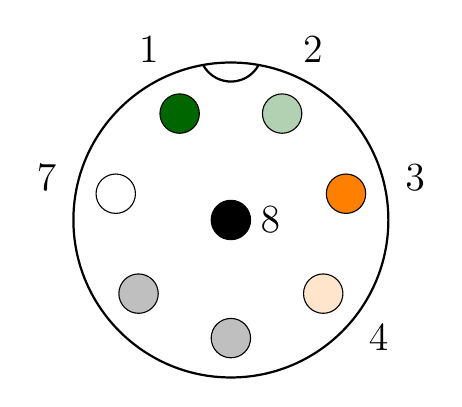
\begin{tikzpicture}
	\def\Ro{2} % Outer connector radius
	\def\Rc{0.75*\Ro} % Radius of pin on connector
	\def\Ri{0.25} % Radius of pins
	\def\Rn{0.4} % Radius of knob
	\def\ang{60} % Angle of knob

	\draw[black, thick] (0,0) circle (\Ro);
	\draw[black, fill=black] (0,0) circle (\Ri);
	\node[xshift=0.5cm] at (0,0) {\Large 8};

	\def\cablecolors{black!60!green, black!60!green!30, orange, orange!20, lightgray, lightgray, white}
	\foreach[count=\i] \col in \cablecolors {
		\def\x{360/7*(\i-1.5)}
		\draw[black, fill=\col] ({sin(\x)*\Rc}, {cos(\x)*\Rc}) circle (\Ri);
		\xintifboolexpr {\i != 5 && \i != 6}
		{\node at ({1.2*\Ro*sin(\x)}, {1.2*\Ro*cos(\x)}) {\Large \i};}
		{}
	}
	\draw [black,thick,domain={-90+\ang}:{-90-\ang}] plot ({\Rn*cos(\x)}, {\Ro + \Rn*cos(\ang)*(1-sin(\ang/5)) + \Rn*sin(\x)});
		
\end{tikzpicture}
	
\end{document}